\section{Designs}
Now that all the different components have been described, it's time to construct some designs they can be used with.

\subsection{Potential Divider}
One of the more simple, yet incredibly important, designs is the potential divider.
This circuit consists of two or more resistors connected up in series.
A voltage can then be measured between each resistor.
This voltage will be proportional to the values of the resistances and the power supply voltage.

\begin{enumerate}
\item Please take two $10K\Omega$ resistors and connect them up as shown
\item Turn on the power supply
\item Use the digital multimeter to measure the voltage at the midpoint
\item Replace R? with a resistor of value $5K\Omega$
\item Measure the voltage at the midpoint
\item Replace R? with a resistor of value $20K\Omega$
\item Measure the voltage at the midpoint
\item What would happen if you replaced R? with a resistor of value $30K\Omega$?
\item Check if you're correct
\end{enumerate}

\subsection{Filters}
Filters are useful circuits which allow particular signals to be subtracted from the input signal.

\begin{enumerate}
\item Construct the filter circuit as shown
\item Turn on the power supply
\end{enumerate}

\subsection{Op-Amp}
There are many different circuits that the operational amplifier can be used in.
Today we will briefly look at some of the simpler ones.

\subsubsection{Comparator}
The differential inputs of the op-amp, and its high gain, means it can be used to detect which of two signals is greater.

The circuit for this is shown below:

\begin{figure}[H]
	\centering
	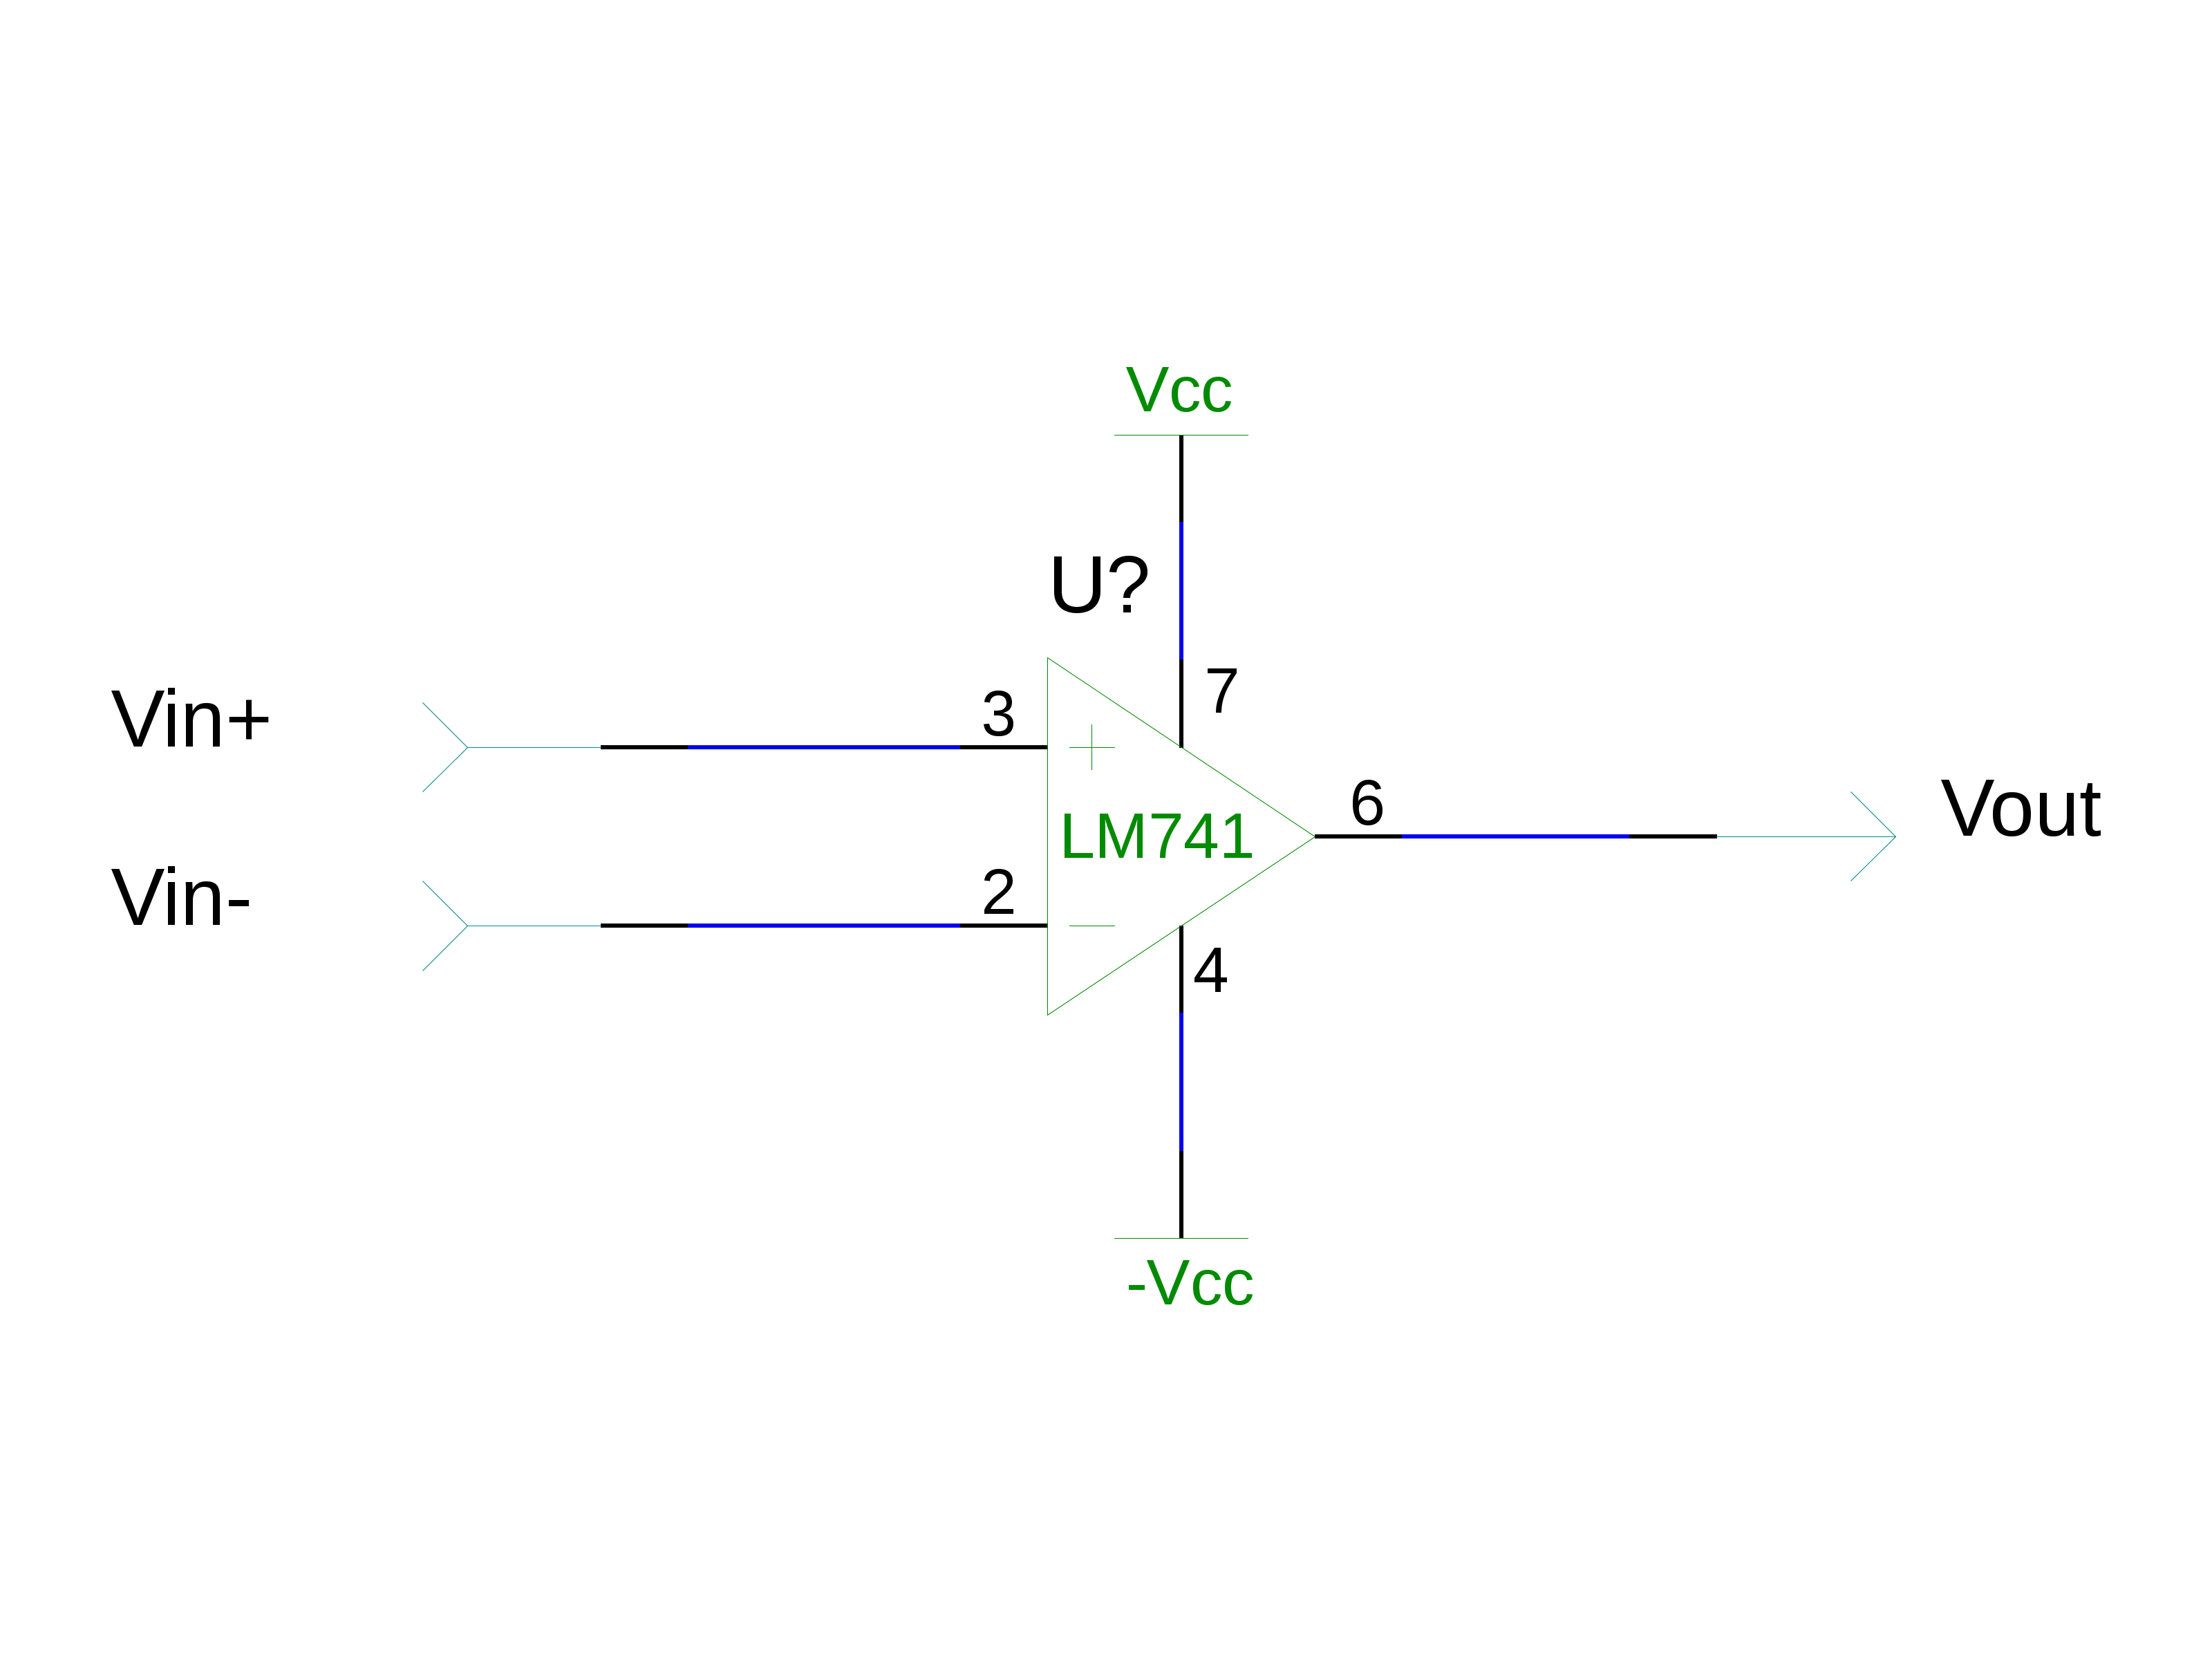
\includegraphics[width=\textwidth]{./images/comparator.png}
	\caption{A comparator circuit}
	\label{fig:comparator}
\end{figure}

\subsubsection{Schmitt Trigger}
The schmitt trigger is an interesting design, as the input signal rises it will give a positive output, however in order to give a negative output the input needs to go significantly lower.

The circuit for this is shown below:

\begin{figure}[H]
	\centering
	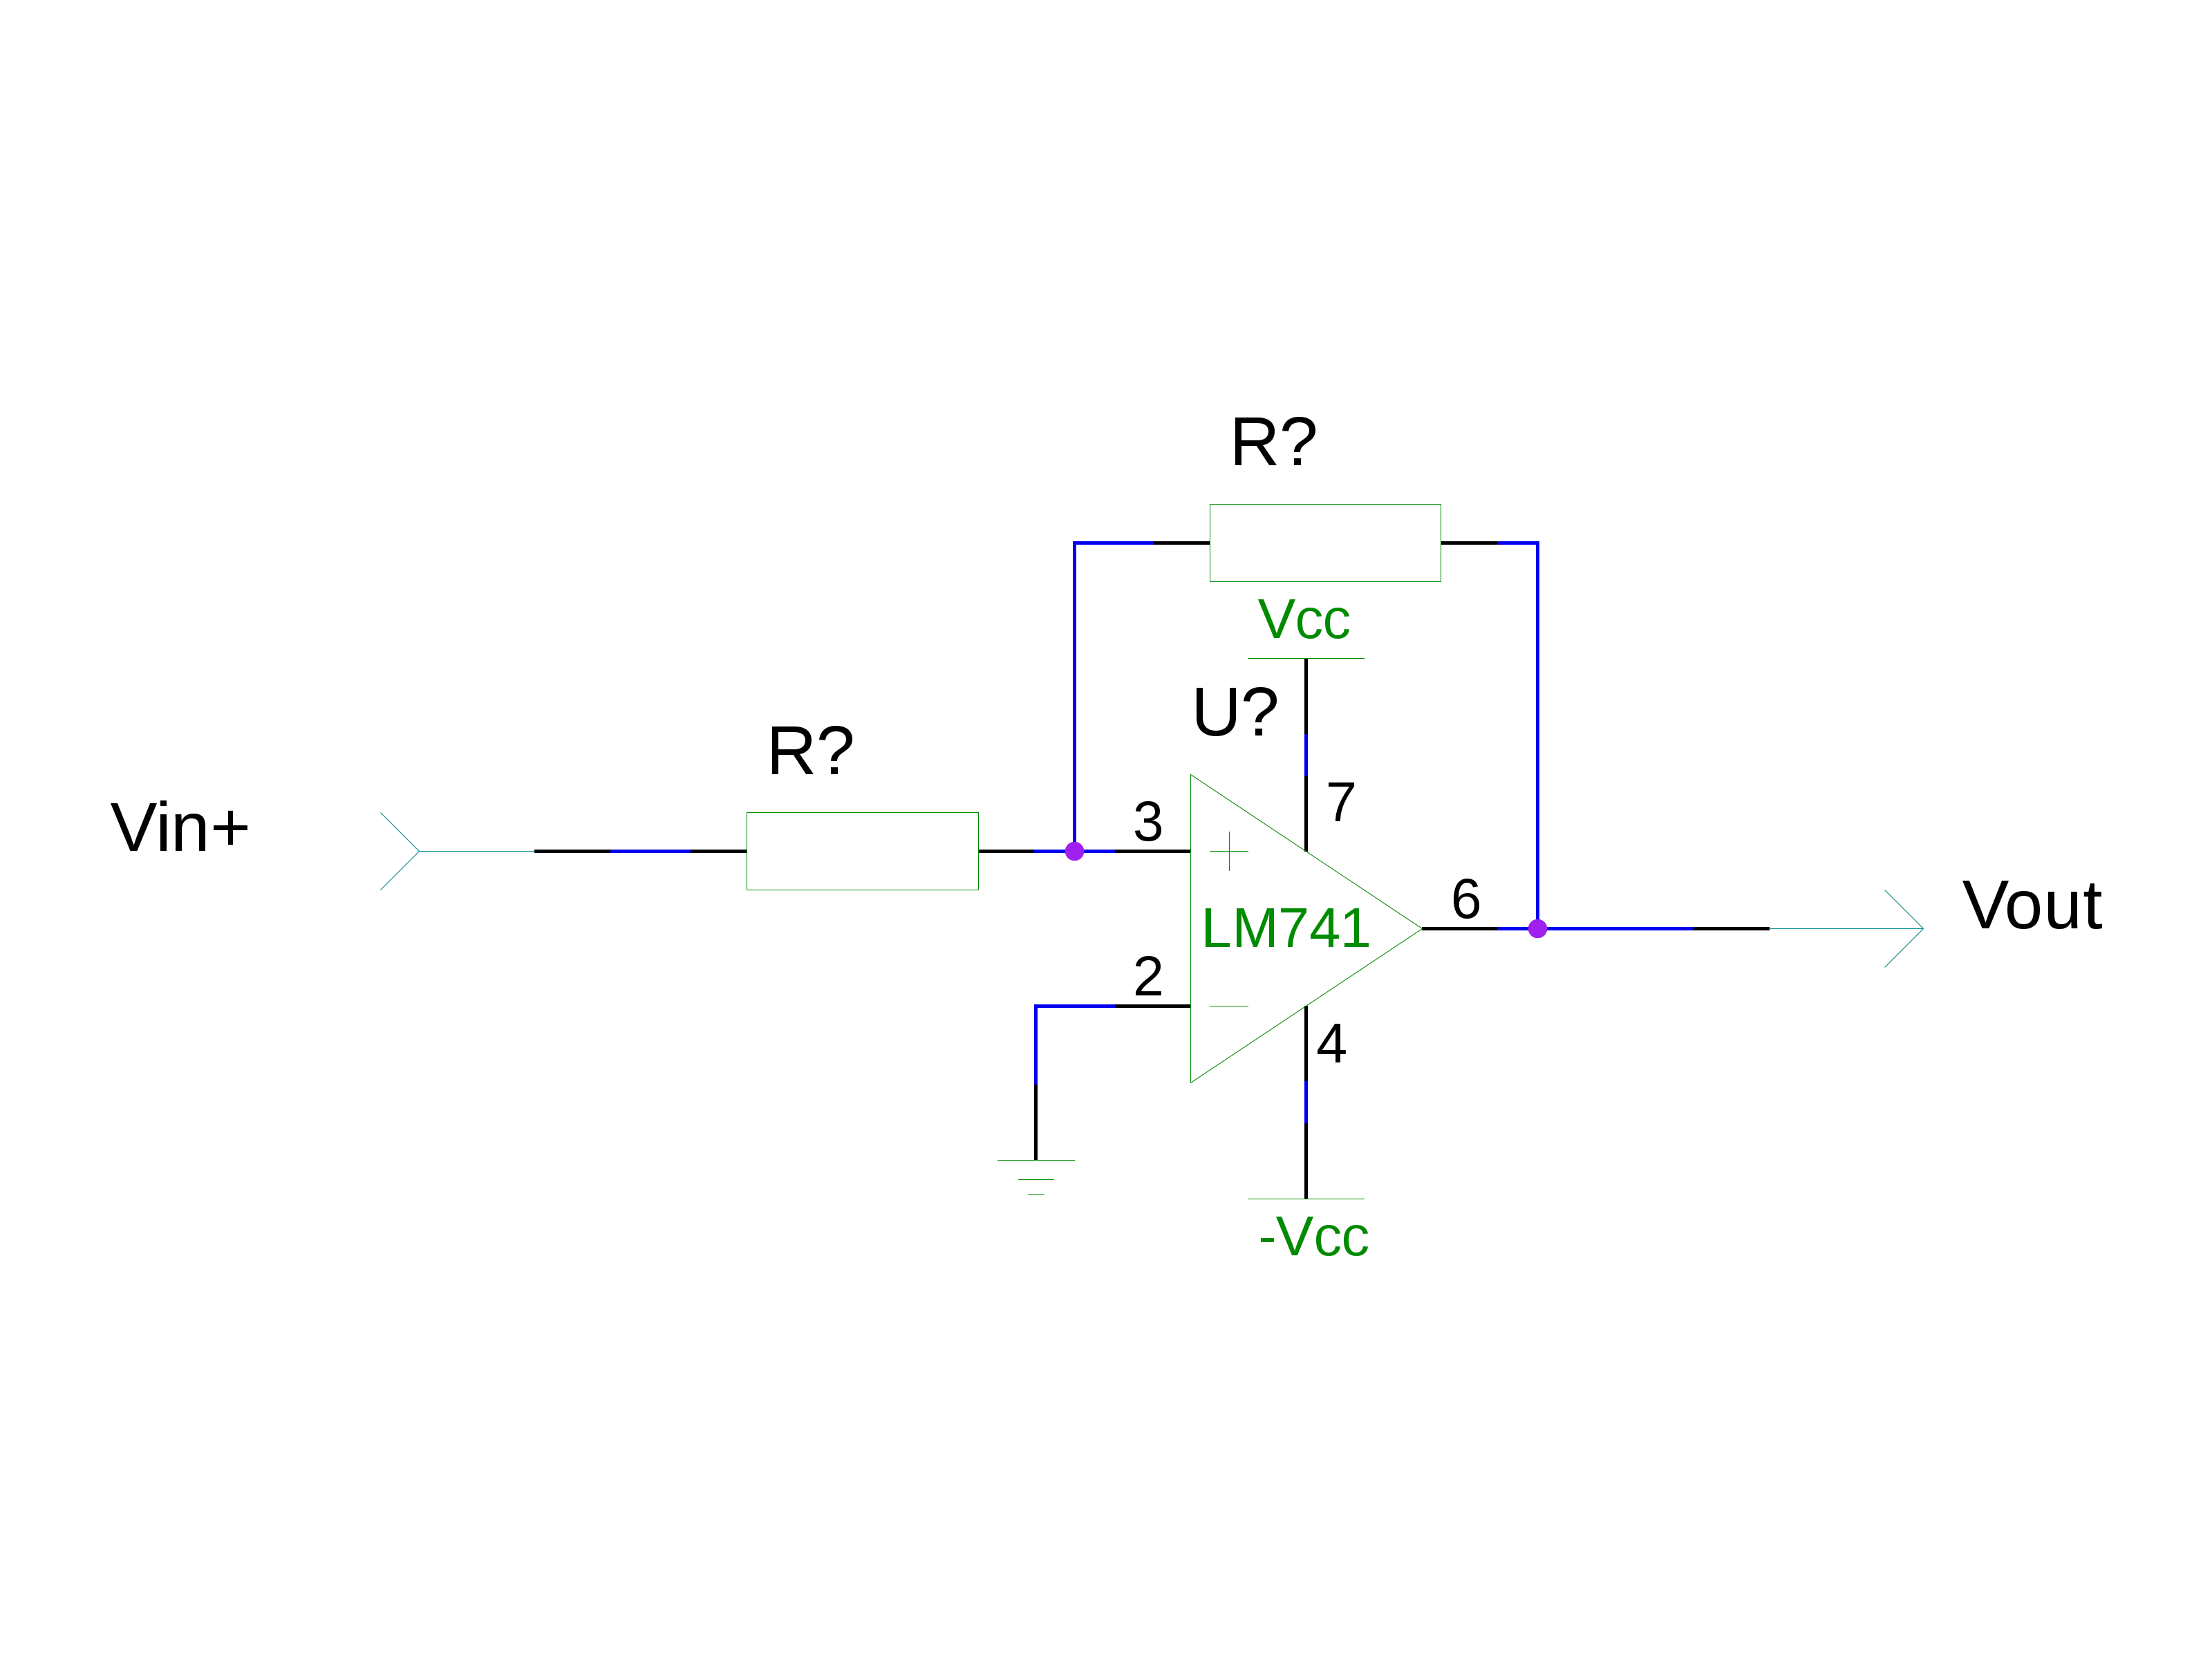
\includegraphics[width=\textwidth]{./images/schmitt.png}
	\caption{A Schmitt Trigger circuit}
	\label{fig:schmitt}
\end{figure}

\subsubsection{Integrator}
The integrator gives an output which rises with a positive input.
With a negative input the output will fall, and with a zero input the output stays constant.

The circuit for this is shown below:

\begin{figure}[H]
	\centering
	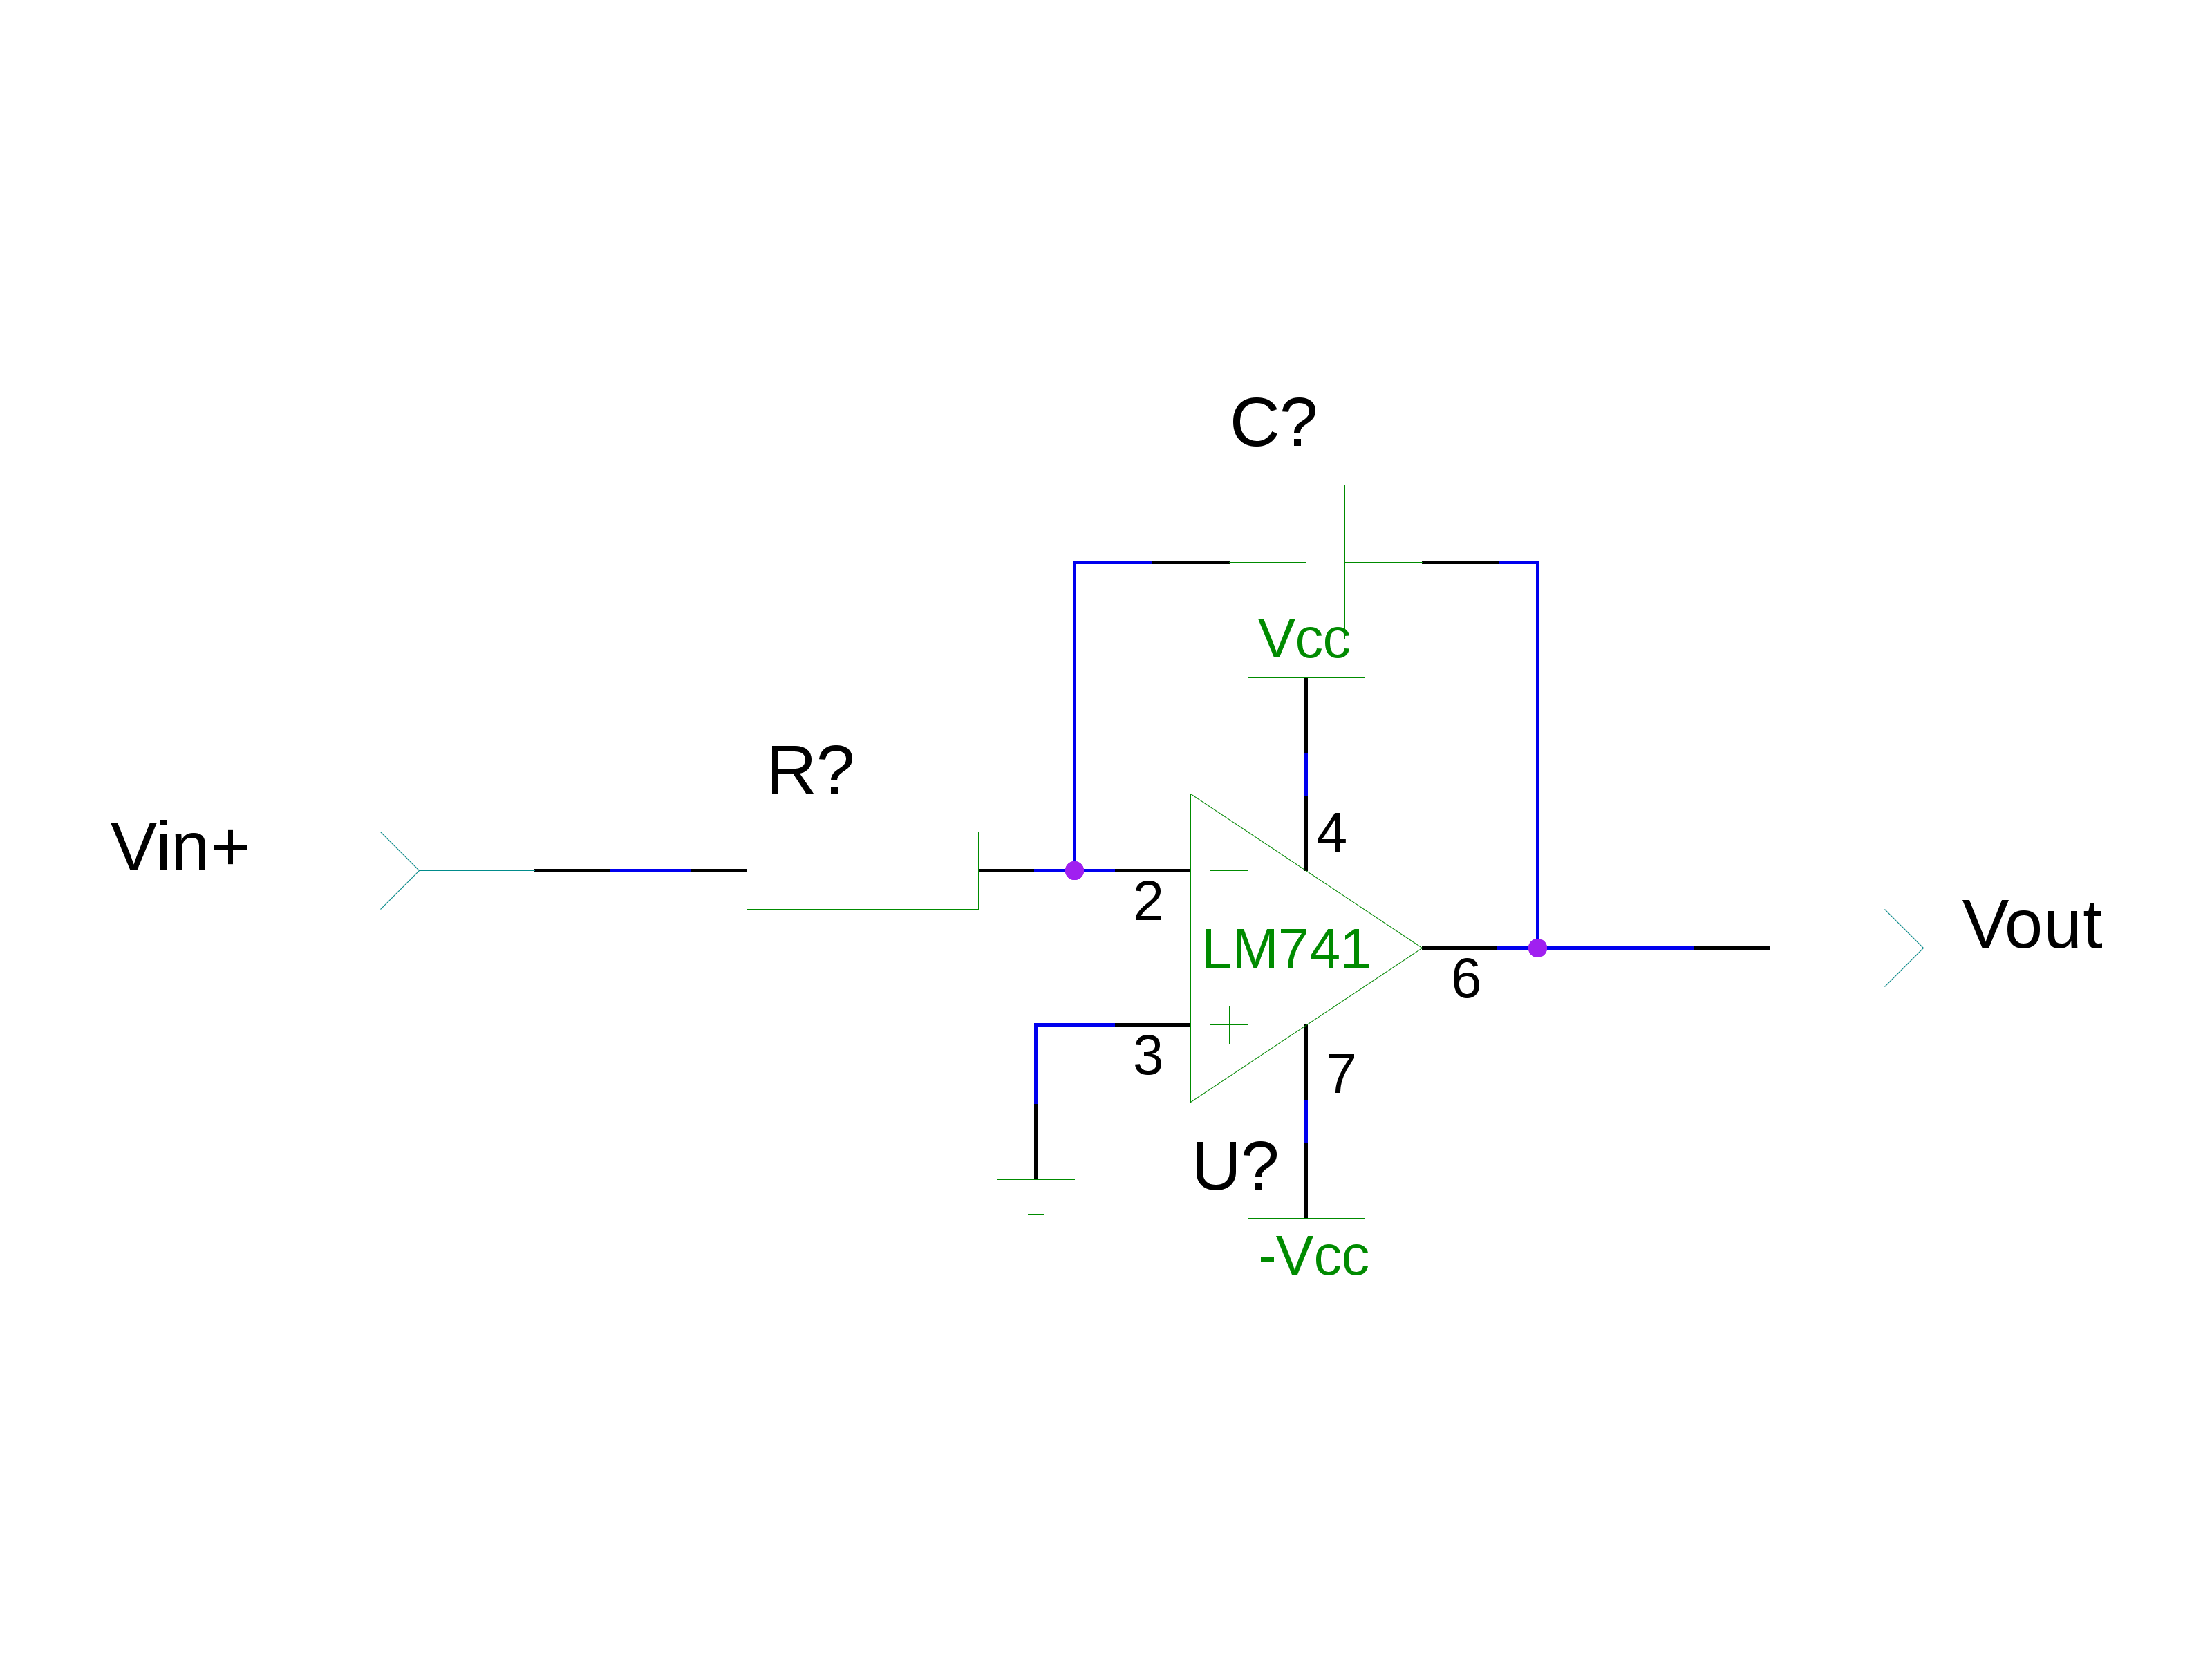
\includegraphics[width=\textwidth]{./images/integrator.png}
	\caption{An integrator circuit}
	\label{fig:integrator}
\end{figure}
